\section{Introductory thoughts}
To start, a small introduction to ADflow's solvers, its history and the initial
state of SST is given.

In the beginning, this solver was called \textit{Standford University
Multiblock (sumb)}. It was intended as a multiblock solver for turbomachinery.
Later on, it was extended to be used in optimizations. For this, an adjoint
solver was needed. As explained in section \ref{sec:gradient_computation}, the
adjoint method needs partial derivatives which are obtained through means of
finite differences and/or automatic differentiation. For the AD part, a tool
called \textit{tapenade}
\footnote{\url{http://www-tapenade.inria.fr:8080/tapenade/index.jsp}} is used.
It automatically differentiates FORTRAN source code. But to get it working, a
lot of the initial structure had to be changed.




\subsection{Flow Solvers}
ADflow has three different solvers available to solve the RANS equations:
\textit{multigrid (MG)}, \textit{Newton-Krylov (NK)} and \textit{Approximate
Newton-Krylov (ANK)}. It is possible to switch between
the different solvers during a solution run. This allows to use each Solver
when it is most efficient: initiate the simulation using multigrid, once a
certain level of convergence is reached, engage the ANK solver an finally
converge the last couple order of magnitudes using the NK Solver.
\footnote{Please note that the ANK solver by itself is sufficient as a startup
strategy and MG is not necessarily needed.}

Multigrid is the baseline solver that was implemented first. It uses either the
Runge-Kutta (RK), or the Diagonalized Diagonally-Dominant Alternating Direction
Implicit (D3ADI) algorithm as a smoother. The turbulence model is solved in a
decoupled manner and using the Diagonalized Alternating Direction Implicit
(DADI) method.

The Newton-Krylov solver solves the nonlinear system of governing equations by
simply using the Newton's method. To solve this linear system, the GMRES
algorithm is used. The turbulence variables are solved in a coupled manner and
thus no other solvers are needed. This method is equivalent to using Euler's
method with an infinite time step. It is most efficient when the solution is
already at the final stages of convergence. If it is used in the early stages,
it most likely stalls.

The Approximate Newton-Krylov is similar to the NK solver in that it also uses
Euler's method. But its time step is adjustable. At the beginning of the run,
it is quite low and thus increases the stability. This allows it to be used
as a startup strategy where the NK solver wouls most certainly fail. The
lower the residual norm is, the more the time step is increased. And as such, it
approaches Newtons' method. It is subdivided into three different sub-solvers:
\textit{First order ANK (ANK)}, \textit{Second Order ANK (SANK)} and
\textit{Coupled ANK (CANK)}. Please note, the combination of both
\textit{Coupled Second-Order ANK (CSANK)} is also possible.

In its base configuration (ANK) uses a first-order routine for the residual
Jacobian and thus only affects convergence, but not the solution accuracy. Once a user defined level of
convergence is reached, the solver switches to an exact Jacobian formulation
(SANK). In these two stages, the turbulence model is solved in a decoupled
manner. Once can choose between a second turbulence-only-ANK solver or the
above mentioned DADI method. It is done this way because the turbulence models
in RANS simulations are notoriously difficult to converge. Once again, when the
residual norm reaches a user-defied level, the coupled mode is enganged. In
that state, only one ANK solver remains which solve the flow and turbulence
variables simultaneously. This helps to improve the convergence in the later
stages. \cite{adflow_solvers}




\subsection{Adjoint Solver}




\subsection{Initial state of SST}
When sumb was developed initially, a multitude of different turbulence models
were implemented such as Spalart-Allmaras (SA) or SST. When the code was
overhauled for optimization, only the SA model was carried over and
differentiated. At that point SST would throw NaNs\footnote{Not a Number} and
crash. Lately, this was fixed to a point where the DADI turbulence solver would
work \footnote{See pull request:
\url{https://github.com/mdolab/adflow/pull/107}}. To summarize, before this
project started, the code for SST was there and could be solved using ANK/SANK
and the decoupled DADI turbulence solver. But nothing was differentiated which
means, the adjoint, NK and coupled ANK solvers were not usable.








\section{Needed changes}
ADflow can parallelize the computation over multiple cpus and computers. It
does this by splitting up the computational domain into blocks. These blocks
may live on different cpus or computers. As those blocks do not live in
isolation and do depended on each other, adjacent blocks need to exchange
information. ADflow uses the \textit{halo cell} approach for this. The idea is
to have imaginary ghost (halo) cells around each block. Then they are filled
with the values from the adjacent blocks. Figure \ref{fig:halo_cells} shows
this idea. One difference to the picture is that ADflow uses two layers of halo
cells.

\begin{figure}[H] \centering
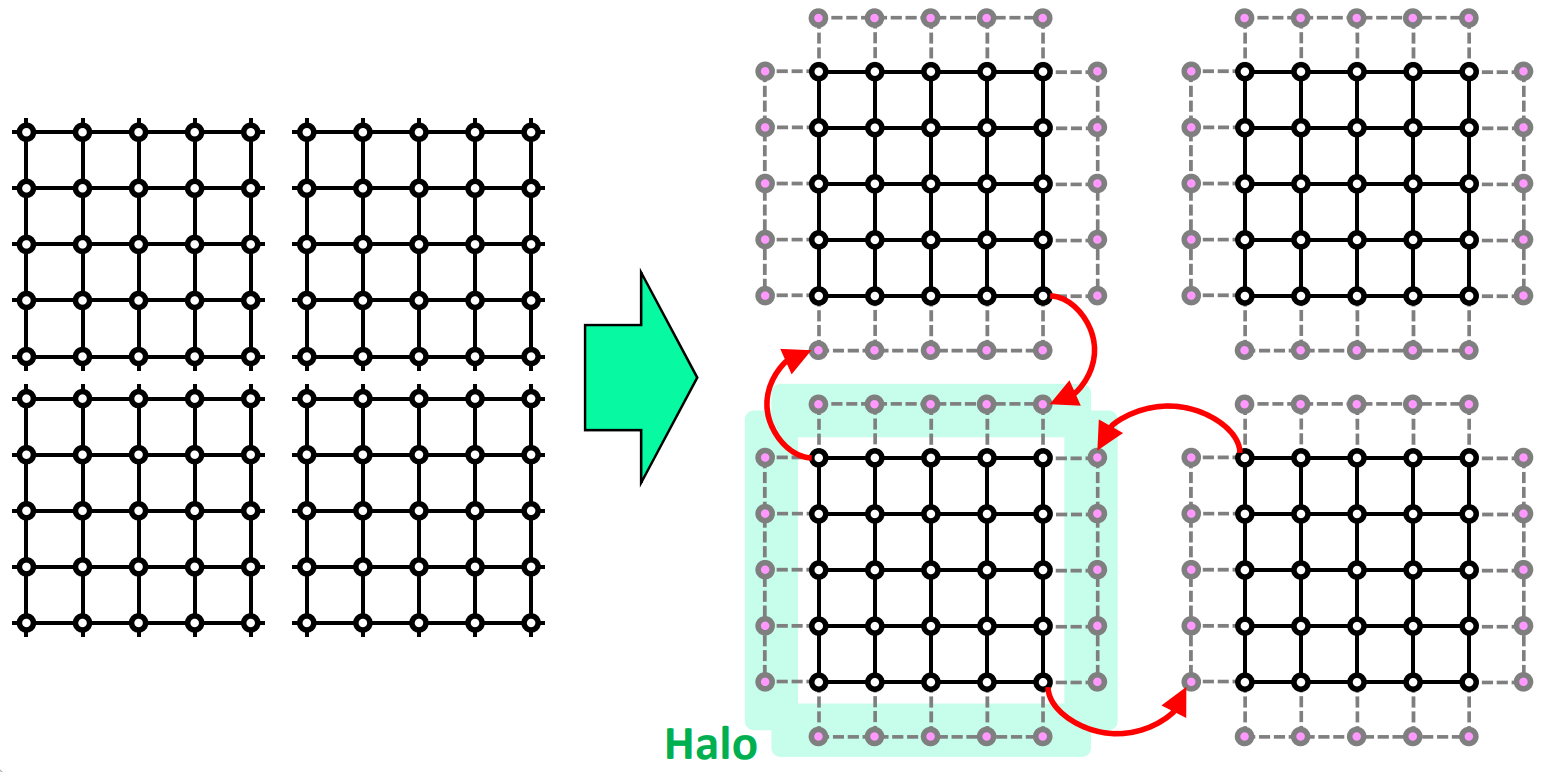
\includegraphics[width=0.7\textwidth]{halo_cells}
    \caption{A block split in 4 (left) and its corresponding halo cells (right)
            \cite{cfd_halo}.}
    \label{fig:halo_cells}
\end{figure}




\subsection{Halo exchange and AD}
This halo exchange is straight forward when one does not care about automatic
differentiation. But we do, and as such, some things need to be considered. The
exchanges is performed using the \textit{Message Passing Interface (MPI)}.
Unfortunately, tapenade can not handle MPI calls. To make this work, the
differentiated code is divided into parts: The \textbf{math heavy} part is
differentiated using tapenade. The \textbf{remaining part} is
hand-differentiated. This is not a big problem as this part mostly consists of
calling the AD part and performing communication. 

The turbulence model is considered a math heavy part that is automatically
differentiated using tapenade. For SA, this was straight forward as there is no
communication going on. But SST has one special case: The blending function
$\mathbf{F_1}$ (equation \ref{eq:f1}). The problem is, it is not a normal
turbulence working variable (such as $k$ or $\omega$) and thus is not exchanged
using existing infrastructure. The developers of sumb fixed this by exchanging
it manually after computing it. This is done in the model itself and was no
problem because nobody intended to AD it. \\

Now the question is: Why was it done this way and how do we get rid of this
intermediate communication?

The first part of the questions might be explained by fact that sumb was
initially developed in the early 2000's. Back then, computing power was more
expensive and computing the same $F_1$ value on different blocks was
wasteful. The cost of communication was negligible in comparison. This did not
really change, but computing power became a lot cheaper. So if it makes AD
easier, it is a good trade to get rid of the communication.

\section{Algorithmic/Automatic Differentiation}

\section{Verification}

\subsection{Testcases}

\subsubsection{NACA 0012}
\subsubsection{RAE 2822}
\subsubsection{Flatplate}
\subsubsection{2D bump}
\subsubsection{3D wing}


\subsection{Partial derivatives}

\subsection{Total derivatives}


